\section{Introduction}
\label{sec:intro}

%% WHAT IS AD HOC DATA?

An {\em ad hoc data format} is any non-standard data format for which
parsing, querying, analysis, or transformation tools are not readily
available.  Despite the increasing use of standard data formats such
as \xml{}, ad hoc data sources continue to arise in numerous
industries such as finance, health care, transportation, and
telecommunications as well as in scientific domains, such as
computational biology and chemistry.  The absence of tools for
processing ad hoc data formats complicates the daily data-management
tasks of IT professionals, who may have to cope with numerous ad
hoc formats even within a single application.  

Common characteristics of ad hoc data complicate even basic tasks,
such as loading ad hoc data into a database system.  Documentation is
often incomplete or inaccurate, and the data itself may contain
syntactic and semantic errors.  Before the data can be processed
reliably by an application, errors must be identified, filtered out,
or corrected, and the cleansed data must be transformed into a
standard loading format.  Surprisingly, few tools exist for supporting
these critical data-management tasks for ad hoc data, and the problems
of handling ad hoc sources are largely ignored by researchers in
data-management domains.

\cut{Once in a standardized format, the data can be directly loaded into a
database or manipulated by standard, widely available tools.}

%% EXAMPLE SOURCES AND CHARACTERISTICS

\cut{\xml{}, for
example, is not ad hoc, because numerous, standard tools for parsing,
querying, and transforming exist for \xml{}.
There are vast amounts of useful data stored in traditional databases
and \xml{} formats, but there is just as much in ad hoc formats.}

The variety of application domains, format characteristics, and
sources of errors make working with ad hoc data challenging.
\figref{figure:data-sources} summarizes several ad hoc sources from the
networking and telecommunication domains at AT\&T and from
computational biology applications at Princeton.  Formats include
ASCII, binary, and Cobol, with both fixed and variable-width records
arranged in linear sequences and in tree-shaped or DAG-shaped
hierarchies.  Common errors include undocumented data, corrupted data,
missing data, and multiple representations for missing values.
Another notable characteristic of these data sources is their large
size: Web server logs, for example, can reach 12GB per week and net-flow
applications over one Gigabit \emph{per second}.

\begin{figure*}
\begin{center}
\scriptsize
\begin{tabular}{@{}|l|l|l|}
\hline
\textbf{Name:} Use & Record Format (Size) 
%& Size
           & Common Errors \\ \hline\hline
\textbf{Web server logs (CLF):}           & Fixed-column ASCII & Race conditions on log entry\\ 
Measuring Web workloads  & ($\leq$12GB/week)  & Unexpected values\\ \hline
\textbf{AT\&T provisioning data (\dibbler{}):} & Variable-width ASCII & Unexpected values \\ 
Monitoring service activation  & (2.2GB/week) & Corrupted data feeds \\ \hline
\textbf{Call detail:}                   & Fixed-width binary &  Undocumented data\\
Fraud detection                         &   (\appr{}7GB/day) & \\ \hline 
\textbf{AT\&T billing data (\ningaui{}):}      & Cobol      & Unexpected values\\ 
Monitoring billing process  &  ($>$250GB/day) & Corrupted data feeds \\ \hline
\textbf{IP backbone data (\darkstar{}):}  & ASCII & Multiple representations \\
{Network Monitoring}       &  ($\ge$ 15 sources,\appr{}15 GB/day)  & of missing values \\
          & & Undocumented data \\ \hline
\textbf{Netflow:}               & Data-dependent number of & Missed packets\\ 
{Network Monitoring}  & fixed-width binary records & \\ 
                      & ($\ge$1Gigabit/second) & \\ \hline
\textbf{Gene Ontology data:}    & Variable-width ASCII & \\
Gene-gene correlations in Magic & in DAG-shaped hiearchy & \\\hline
\textbf{Newick data}              & Fixed-width ASCII & Manual entry errors \\
Immune system response simulation & in tree-shaped hierarchy 
& \\
\hline
\end{tabular}
\normalsize
\caption{Selected ad hoc data sources.}
\label{figure:data-sources}
\end{center}
\end{figure*}

%% WHY IS PROCESSING IT HARD?
%% No control of source or target format

In addition to poor documentation and error-prone data sources, other
common characteristics of ad hoc data make basic processing tasks
challenging.  For example, a data analyst cannot control the format of
the ad hoc data at its source nor at its final destination, for
example, in a database.  The data arrives ``as is'', and the analyst
who receives it can only thank the supplier, not request a more
convenient format.  Once an analyst has the data, a common task is
converting the source format to a standard database loading format.
This transformation proceeds in three stages.  First, the analyst
writes a parser for the ad hoc format, using whatever (in)accurate
documentation may be available.  Second, he writes a program that that
detects, corrects or deletes erroneous data records, selects records
of interest, and possibly normalizes records into a standard format,
for example, by reordering, removing, or transforming fields.
Unfortunately, the parsing, error handling, and transformation code is
often tightly interleaved.  This interleaving hides the knowledge of
the ad hoc format obtained by an analyst and severely limits the
parser's reuse in other applications.

\cut{A common phenomenon is for a
field in a data source to fall into disuse.  After a while, a new
piece of information becomes interesting, but compatibility issues
prevent data suppliers from modifying the shape of their data, so
instead they hijack the unused field, often failing to update the
documentation in the process.}

%% Sources, meaning, and handling of errors
Another challenge in processing ad hoc data is handling the variety of
error kinds and the variety of application-dependent strategies for
handling errors.  Some of the sources of errors that we have
encountered in ad hoc sources include malfunctioning equipment, race
conditions on log entry~\cite{wpp}, presence of non-standard values to
indicate ``no data available,'' human error when entering data, and
unexpected data values.  A wide range of responses are possible when errors
are detected, and they are highly application dependent.  Example
responses include haulting processing and altering a human operator, to
partitioning error from error-free records for examination off-line, to
simply discarding erroneous or unexpected values.  One of the most
challenging aspects of processing ad hoc data is that erroneous data
is often more important than error-free data, because it may indicate,
for example, that two systems are failing to communicate.  Writing
code that is reliably \emph{error aware}, however, is difficult and
tedious.

%% High-volume
Another challenge is efficient, error-aware processing of 
data sources that are high volume.  AT\&T's call-detail stream contains roughly 300~million
calls per day requiring approximately 7GBs of storage space.  Although
this data is eventually archived in a database, analysts mine it
profitably before such archiving~\cite{kdd98,kdd99}.  More
challenging, the \ningaui{} project at AT\&T accumulates billing data
at a rate of 250-300GB/day, with occasional spurts of 750GBs/day.
Netflow data arrives from Cisco routers at rates over a Gigabit per
second~\cite{gigascope}!  Such volumes require that the data be
processed without loading it into memory all at once.  More
importantly, flexible error-response strategies are necessary for
high-volume sources, so that processing is not haulted or delayed when
errors are detected.

%% EXISTING SOLUTIONS

Today, people tend to use \C{} or \perl{} for this task.
Unfortunately, writing parsers, transformations and printers this way
is tedious and error-prone, complicated by the lack of documentation,
convoluted encodings designed to save space, the need to produce
efficient code, and the need to handle errors robustly to avoid
corrupting down-stream data.  Moreover, the parser writers' hard-won
understanding of the data ends up embedded in parsing code, making
long-term maintenance difficult for the original writers and sharing
the knowledge with others nearly impossible.

% The goal of this paper is to describe a new language for efficient and
% reliable computing with ad hoc data.  More specifically, we describe a
% high-level programming language, \datatype{}, that comes with
% intrinsic support for processing ad hoc data.  Our programming
% language will use the rich data descriptions both as directives for
% parsing ad hoc data sources and as types for describing
% representations of ad hoc data within the programming environment.  In
% addition, a critical facet of our language will be its support for
% {\em error-aware computing}.  Our error-aware infrastructure will
% allow programmers to conveniently verify correctness of data relative
% to a description or alternatively detect data errors and handle them
% in domain-specific ways.  Finally, we will be sure our language design
% is founded on strong programming language principles by studying its
% type system and metatheory extensively.

%% OUR SOLUTION

\cut{
%% This material moved to the intro?
\datatype{} is more than a data description language. It is also a
functional programming language with extensive support for data
transformation. Most importantly, \datatype{} is not merely a
combination of these two language elements - data description and
transformation - but a synthesis.  The meta-data learned during the
process of parsing the data based on its description is not lost once
the parsing is finished, but instead plays a prominent role in the
programmatic elements of the language. As we are particularly
concerned with error-related meta-data, we term this synthesis
``error-aware computing.''
}

Solution: Data description Language + transform language
Combine data description language with a transform language.
\pads{} is bound to C. However, functional programming languages are
better suited to the task of data tranformation. We therefore propose
a new language, \datatype{}, that combines a data description language
based on the style of ML types (and datatypes) with a functional data
transformation language. 

Our contributions are twofold. First, we propose an ML-style syntax
for the \pads{} data description language, based on type definitions
and {\em(polymorphic coming soon?)} parameterized recursive datatypes
(support for recursive datatypes is new to the \pads{} language, based
on recent results in our other work). This new syntax has a number of
advantages. It is more concise than the C-style encoding and more
naturally suited to describing recursive datatypes. Most importantly,
the new syntax is much more appropriate for transformation language
proposed below, which is based heavily on pattern-matching and data
constructors.

Our second contribution is the data transformation language itself.
{\em \pads{} is not a programming language.}  It merely generates
libraries that can be used by \C{} programmers.  \C{} is a very
low-level language that makes transforming ad hoc data awkward,
cumbersome and potentially error-prone.  More importantly, it provides
no intrinsic support for dealing with the errors that appear in ad hoc
data.  In addition, \C's type system and operational model provide no
support for checking the rich invariants found in ad hoc data either
at run time or at compile time.  In contrast, \datatype{} is a
high-level language with an elegant and convenient syntax for
data-driven programming, intrinsic support for handling errors and
intrinsic mechanisms for checking data invariants at run time {\em
  coming soon: and a sophisticated type system for enforcing data
  invariants at compile time}. 

%% CONTRIBUTIONS

At its core, \datatype{} is a functional language with standard
features such as pattern matching and higher-order functions, which we
view as critical to supporting data-driven transforms. In addition,
\datatype{} allows programmers to enforce semantic constraints on
data by using \datatype{} descriptions as a special form of runtime
contracts. The basic values of the language will be pairs of data
items and their corresponding meta-data. For each data item, the meta
data will include, among other things, descriptions of the error
content of the data item. Through the type system, the language will
ensure that data and associated meta data are kept in sync. This
property (which we call ``error-aware computing'') enables three
critical language features.
\begin{enumerate}
\item Safe, error-transparent transformations
\item Error querying - analyst can extract detailed picture of data
  error profile.
\item Flexible, programmatic repair of faulty records - analyst can
  choose when in the processing stream to address errors, rather than
  being forced to drop all faulty records at the beginning of the process.
\end{enumerate}

\cut{Consequently, tools for
ad hoc data should provide constructs that are \emph{error aware}.}

Before we talked about two contributions:-- a universal data
description language based on polymorphic, recursive anddependent data
types-- the transformation languageThere might be a third:--
collection and analysis a variety of different examples of ad hoc
datafrom widely differing domains (networking to genomics).  The
analysis of thedifferent sorts of ad hoc data is a substantial
contribution.  It helps usunderstand what is required and what is not.

\subsection{\datatype{} Architecture}

\begin{figure}[tp]
  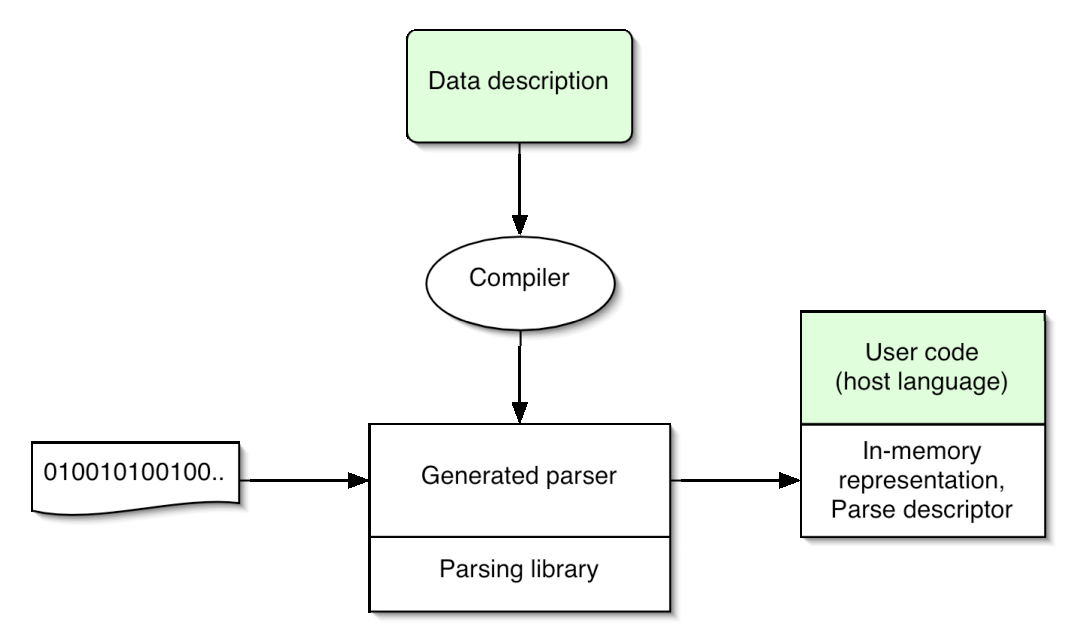
\includegraphics[height=3in,width=5in]{architecture}
%  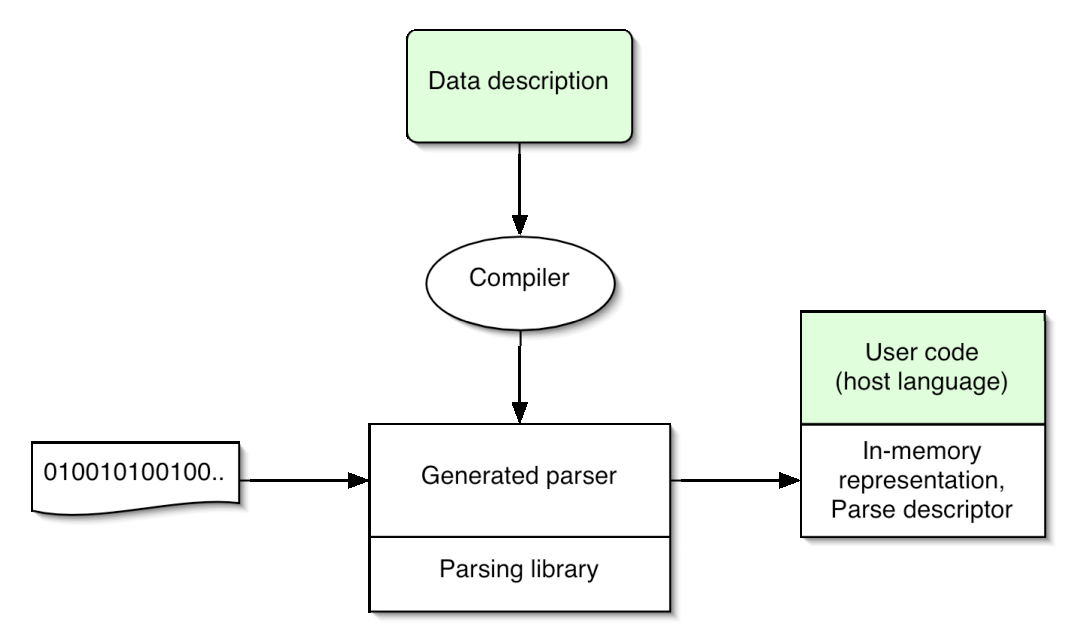
\includegraphics{architecture.eps}
\label{fig:pads-arch}
\caption{The \pads{} Architecture}
\end{figure}

In the next section, we will describe, in detail, the \pads{} approach
to data and meta data (inherited by \datatype{}), the \datatype{}
syntax for data description, and illustrative examples. Next, in
section~\ref{sec:data-transformation} we will elaborate on
\datatype{}'s support for data transformation, including design,
syntax, brief overview of the semantics and some examples.
Section~\ref{sec:implementation-techniques} will discuss our proposed
implementation techiniques, and section~\ref{sec:related-work} the
related work. A discussion of conclusions and future work is included
in section~\ref{sec:conclusion}.

